\documentclass[runningheads]{llncs}
\usepackage[T1]{fontenc}
\usepackage{graphicx}
\usepackage{subcaption}
% \usepackage[UTF8]{ctex} % CTeX package removed for English compilation
\usepackage{enumitem}
\usepackage{tabularx}
\usepackage{booktabs}
\usepackage{multirow}
\usepackage{makecell}

% 居中对齐
\newcolumntype{C}[1]{>{\centering\arraybackslash}m{#1\textwidth}}

% 左对齐
\newcolumntype{L}[1]{>{\raggedright\arraybackslash}m{#1\textwidth}} 

% 右对齐
\newcolumntype{R}[1]{>{\raggedleft\arraybackslash}m{#1\textwidth}}

\bibliographystyle{splncs04}

\AtBeginDocument{%
  \providecommand\BibTeX{{%
    Bib\TeX}}}

\begin{document}

\title{The Impact of Haptic Feedback on Physics Learning Outcomes in Immersive Gesture-Based Learning Environment}

\author{Anonymous Author(s)}

\maketitle

\begin{abstract}
With the advancement of gesture tracking technology, Virtual Reality (VR) based gesture interaction environment offers an intuitive operational experience for physics experiment instruction. However, the lack of haptic feedback in traditional virtual scenes makes it difficult for students to establish a connection between "gestural operation and physical perception," which constrains learning immersion and the depth of knowledge comprehension. This study investigates the impact of haptic feedback on physics learning outcomes in immersive gesture-based learning environment, designing an empirical study based on high school physics experiments. Using a multimodal data analysis approach that integrates physics knowledge tests, subjective questionnaires, and objective physiological metrics, this research systematically explores the differential effects of haptic feedback on interactive experience and knowledge acquisition. The results show that gesture interaction integrated with haptic feedback (1) significantly improves the learner's interactive experience, specifically by enhancing learning motivation (p<0.001) and immersion (p<0.001) without significantly increasing cognitive load (p=0.602); and (2) does not reach statistical significance in improving learners' knowledge acquisition (p=0.087), but shows a positive trend with a medium effect size (|r|=0.303). This study provides empirical evidence and pathways for optimizing the design of physics experiment instruction in immersive gesture-based learning environments.

 \keywords{Immersive Physics Education \and Gesture Interaction \and Haptic Feedback \and Learning Outcomes \and Multimodal Data}
\end{abstract}
 
\section{Introduction}
The core objective of physics experiment instruction is to establish a cognitive link from "phenomenon observation to physical laws to abstract concepts" through hands-on practice\cite{civelek2014effects,bao2019physics,freeman2014active}. However, traditional experiments are constrained by factors such as equipment wear and tear and spatiotemporal limitations, making it difficult to meet personalized learning needs\cite{yang2007impact,ma2023investigation}. Virtual Reality (VR) technology, through immersive interaction enabled by gesture tracking, offers a potential solution to this dilemma\cite{yang2019gesture}. For instance, students can explore the laws of friction by grasping a virtual slider or observe changes in electric current by adjusting circuit components with hand gestures. Nevertheless, existing VR physics experiments generally lack haptic feedback. This means that when students operate a spring dynamometer or feel the weight of an object, they rely solely on visual judgment, failing to form a closed loop of embodied cognition connecting "the effect of force—muscular perception—physical concept"\cite{giri2021application}.

This perceptual deficit directly impacts learning outcomes. On one hand, because learners cannot receive haptic feedback equivalent to that in real experiments, they struggle to build the association between "gestural operation and physical perception," causing their sense of immersion to remain at the visual level\cite{app14114935}. On the other hand, the absence of haptic information may weaken the deep understanding of physical concepts. For example, when exploring the principle of buoyancy, students cannot perceive the relationship between the magnitude of buoyant force and the volume of displaced liquid through touch, relying instead on formulaic derivation, which reduces the intuitiveness of knowledge construction\cite{neri2024enhancing}. Furthermore, existing research indicates that multisensory stimulation can enhance subsequent recall and significantly improve learning efficiency, which indirectly corroborates the negative impact of the aforementioned haptic perception deficit on learning outcomes\cite{murray2023crossmodal}.

This study focuses on the mechanism of haptic feedback in immersive gesture-based learning environments. Using high school physics experiments as the context, it employs a multimodal analysis approach that integrates neurophysiological data, objective test scores, and subjective questionnaires to systematically investigate the differential effects of haptic feedback on interactive experience and knowledge acquisition. The findings reveal that while haptic feedback did not significantly improve knowledge test scores (p=0.087), it optimized the learning process by enhancing learning motivation (p<0.001) and immersion (p<0.001) without increasing cognitive load (p=0.602). This result offers a new perspective for physics experiment instructional design: the value of haptic feedback lies not only in knowledge transmission but also in stimulating deep cognitive engagement through embodied interaction.


\section{Related Work}
\subsection{Gesture Interaction in VR Learning} 

As a core feature of VR education, gesture interaction enables human-computer dialogue through natural movements, significantly enhancing learning engagement\cite{johnson2017embodied}. For example, in a physics circuit experiment, students can adjust resistance by a pinching gesture and observe the trend of current change with a sliding gesture. This "what you see is what you control" interaction model is more intuitive than traditional mouse operations\cite{philippe2020multimodal}. Research shows that gesture interaction can reduce cognitive load because learners do not need to memorize additional key commands, allowing their attention to be focused on the experimental principles themselves \cite{hostetter2023comparing}.

However, a significant problem with VR gesture interaction is the lack of haptic feedback, which leads to operational distortion. For example, when grasping a virtual object, one cannot perceive changes in weight, which affects the intuitive understanding of physical quantities\cite{park2025ultraboard}. Previous studies have pointed out that haptic feedback, as a supplementary sensory channel, can significantly enhance the realism and operational precision of virtual experiments. In the context of physics education, appropriate haptic feedback not only helps students establish an embodied cognitive link of "action-perception-physical law" but also reduces the cognitive load caused by operational uncertainty\cite{zhai2021study}. Additionally, the role of haptic feedback in enhancing learning motivation and immersion has garnered attention. Relevant literature indicates that embodied interactive experiences can stimulate students' desire for exploration and participation, enhancing their engagement in virtual experiments\cite{kontra2015physical,lindgren2016enhancing}. Especially in abstract subjects like middle school physics, transforming abstract physical quantities into perceivable operational experiences through haptic feedback helps students form more intuitive and profound knowledge representations\cite{han2011incorporating}.

In summary, the integration of gesture interaction and haptic feedback has become an important direction for improving the effectiveness of VR physics education. However, systematic empirical research on its mechanisms and learning outcomes is still limited and requires further in-depth exploration.

\subsection{Subjective and Objective Evaluation}
The most common tool for subjective evaluation is the questionnaire, which quantifies the learning experience through learner self-reports, with data primarily collected via survey forms. These instruments typically include scales for cognitive load\cite{sweller1988cognitive}, learning motivation\cite{keller1987development}, and immersion\cite{sherman2003understanding}, used to assess the learner's psychological state in the virtual environment. However, subjective scales have certain limitations: on one hand, learners' self-reports can be influenced by factors such as emotions and social desirability, leading to data bias; on the other hand, scales can usually only reflect the learner's perception of the experience and cannot directly measure the physiological basis of cognitive processes\cite{solano2024interoceptive}.

Objective evaluation, in contrast, focuses on observable behaviors\cite{mayer2003nine} and neurophysiological signals. For instance, at the behavioral level, metrics such as task completion rate, number of operational errors, and interaction duration are recorded to quantify the mastery of learning skills. At the neurophysiological level, cognitive load and emotional states are analyzed using physiological data like electroencephalography (EEG) and heart rate variability (HRV)\cite{liu2023fusion,brugnera2016cortical,kobayashi2025pilot}. This method can provide objective, real-time information about cognitive states, reflecting the learner's implicit cognitive processes, but it has a higher collection cost and more complex data analysis\cite{diarra2025systematic}.


\subsection{Multimodal Fusion Evaluation}
The evaluation of immersive learning effectiveness must break through the limitations of a single dimension, integrating multimodal subjective and objective data for a comprehensive analysis to fully reveal its impact mechanisms\cite{tao2025learning,sharma2020multimodal}. Among these, subjective data focuses on the learner's perceived experience and self-reports, while objective data concentrates on quantifiable behavioral performance and physiological responses. The two corroborate each other, jointly constructing a scientific interpretation of learning outcomes\cite{dengel2018immersive}.

In recent years, the fusion analysis of multimodal data has become a research trend. Combining "high cognitive engagement indicated by EEG signals" with "improvement in task completion rates" and "high satisfaction reported subjectively" can more rigorously validate the promotional effect of immersive environments on learning outcomes\cite{DUBOVI2022104495}. This multi-dimensional evaluation framework not only objectively describes the effects of immersive physics learning but also provides a deeper analysis of the internal connections among "environment design, cognitive processes, and learning results," offering empirical evidence for optimizing immersive learning systems\cite{lindgren2016enhancing,liu2024behavioral}.

\section{Experimental Design}
\subsection{Research Content and Hypotheses}
This study focuses on the impact of haptic feedback on physics learning outcomes in immersive gesture-based learning environment, proposing the following hypotheses:

\begin{enumerate}[label={$\bullet$}]
 \item H1: In immersive gesture-based learning environment, appropriate haptic feedback can improve learners' knowledge acquisition.
 \item H2: In immersive gesture-based learning environment, appropriate haptic feedback can enhance learners' interactive experience.
\end{enumerate}

\subsection{Participants and Environment}

We recruited 64 second-year high school students from XXX High School, with an average age of 16.3±0.8 years. All students had already learned the basic theory of conservation of momentum, possessed similar educational backgrounds, and had comparable prior knowledge levels. The experimental environment is shown in Figure \ref{fig:experimental-show}.

\begin{figure}
 \begin{subfigure}{0.32\linewidth}
  \centering
  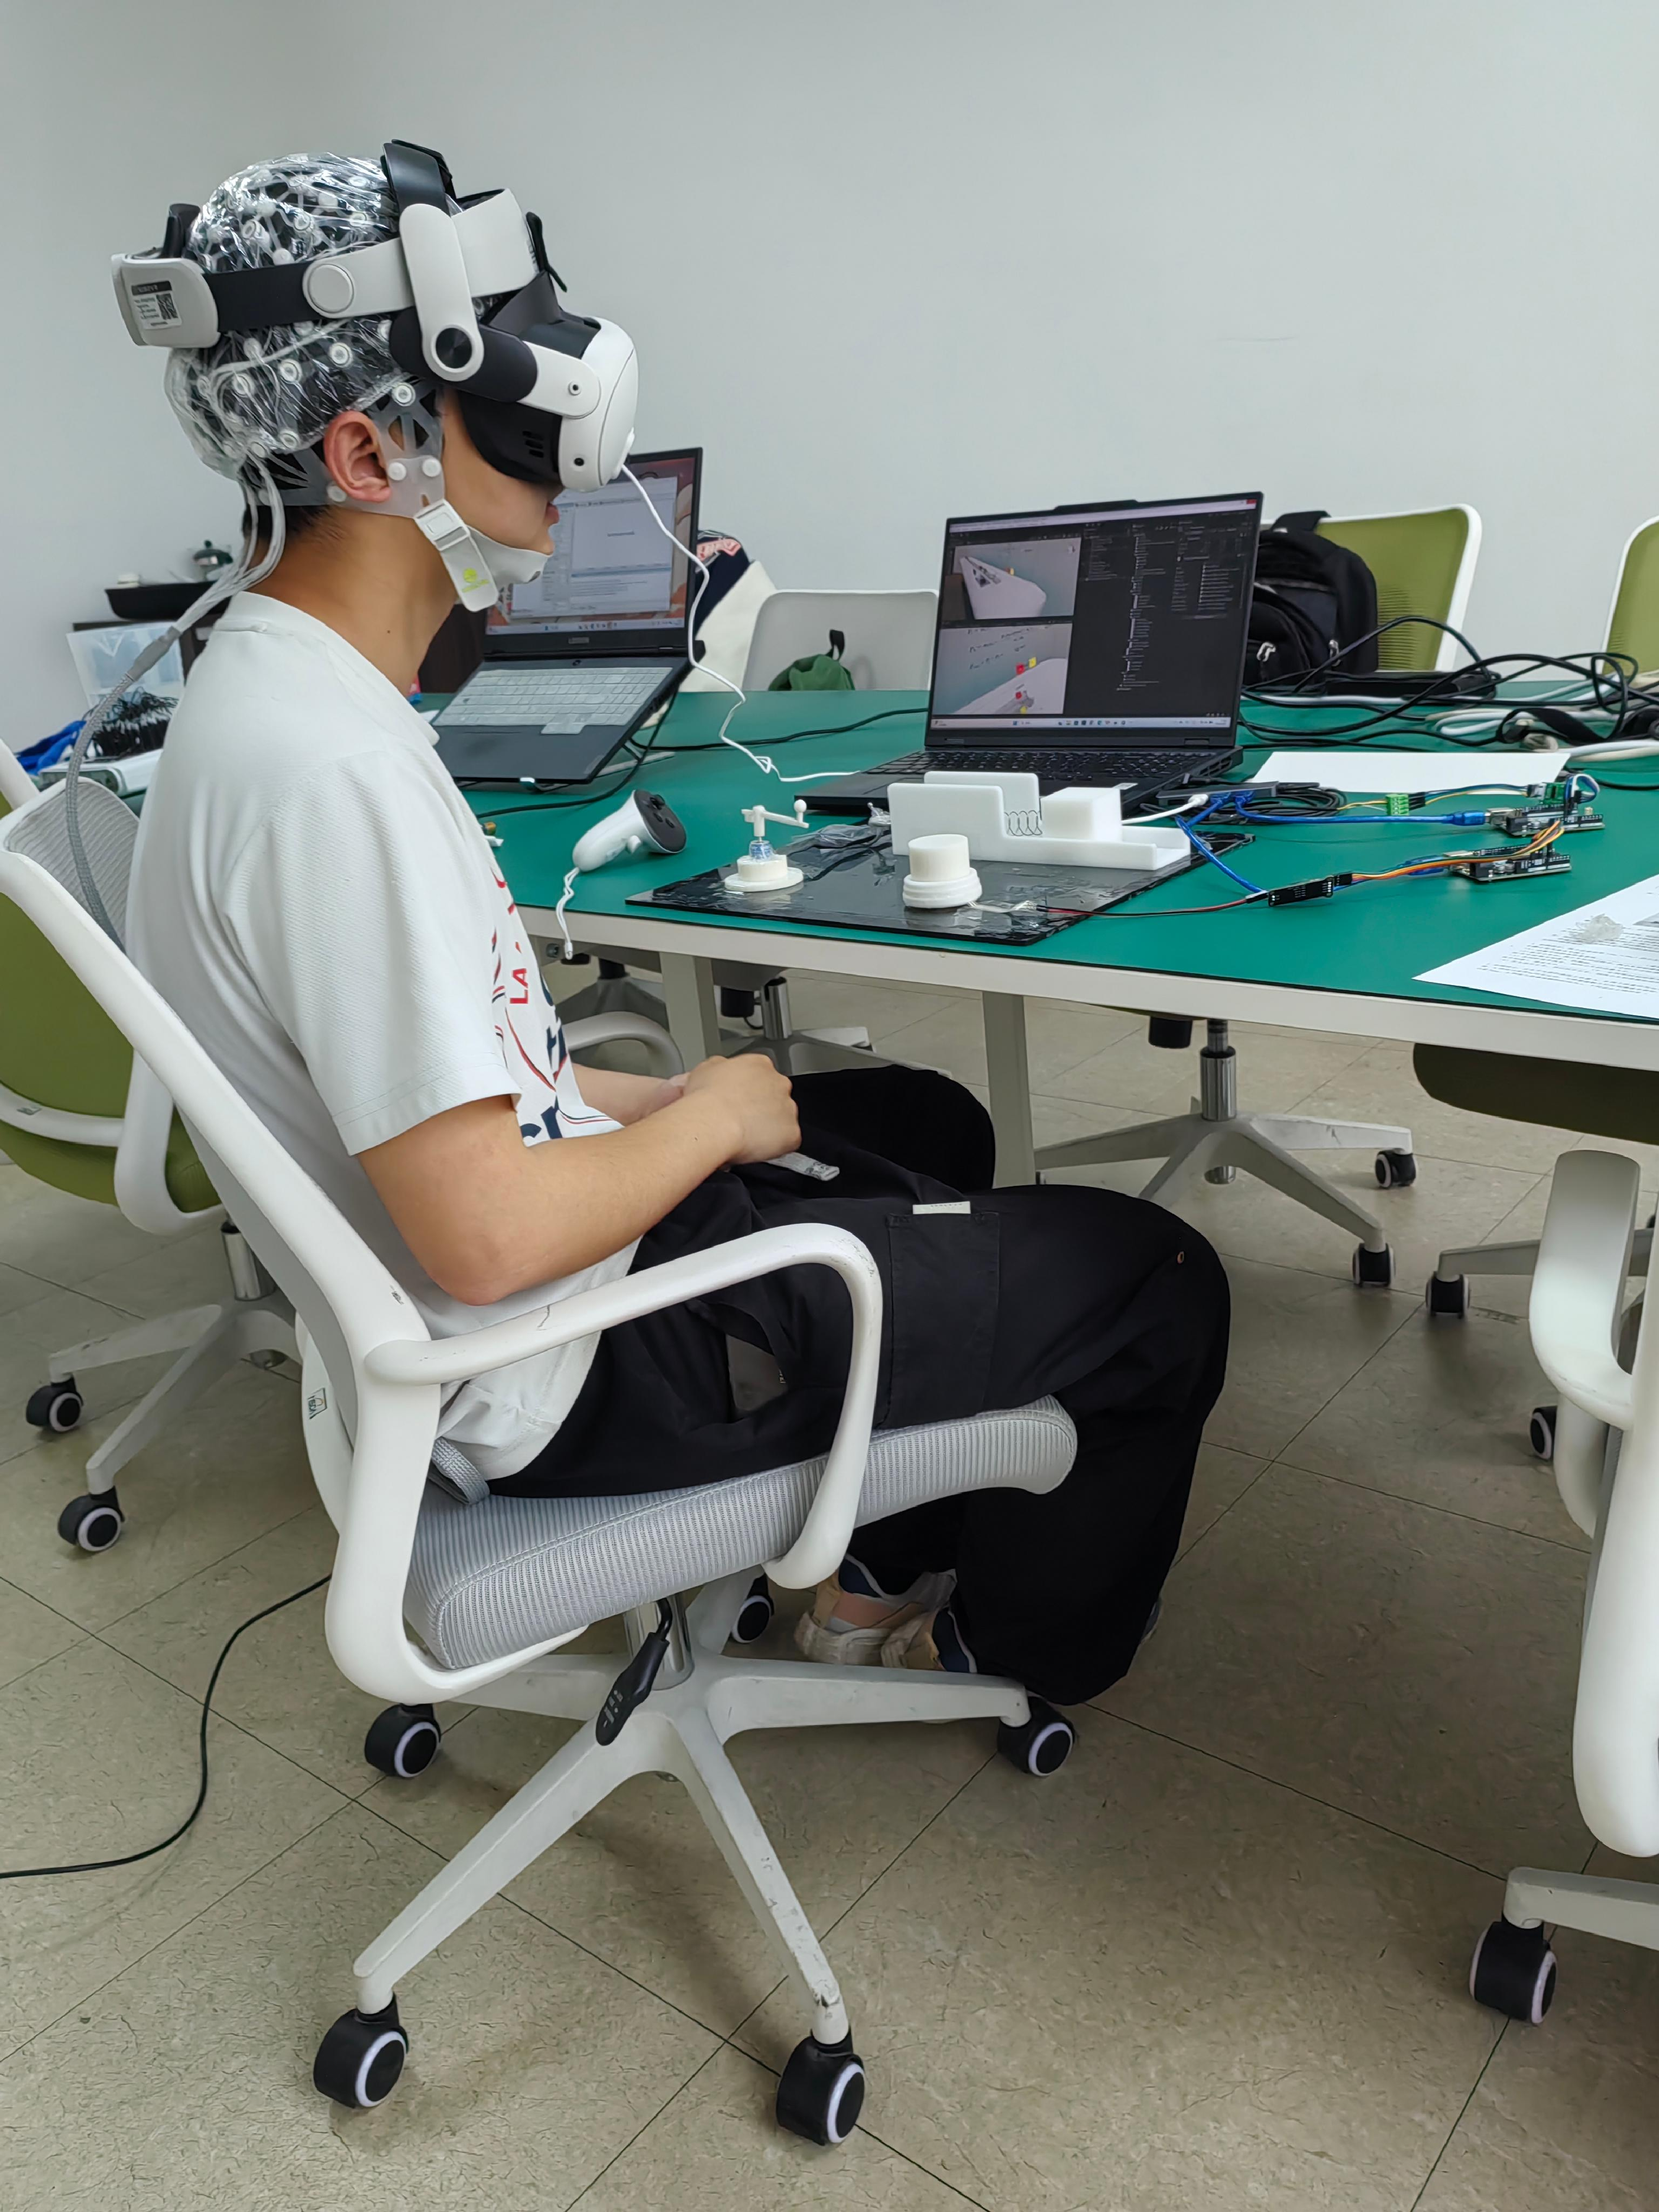
\includegraphics[width=\linewidth]{image/experiment-environment.pdf}
  \caption{Evaluation environment}
  \label{fig:experimental-introduction}
 \end{subfigure}
 \hfill
 \begin{subfigure}{0.64\linewidth}
  \centering
  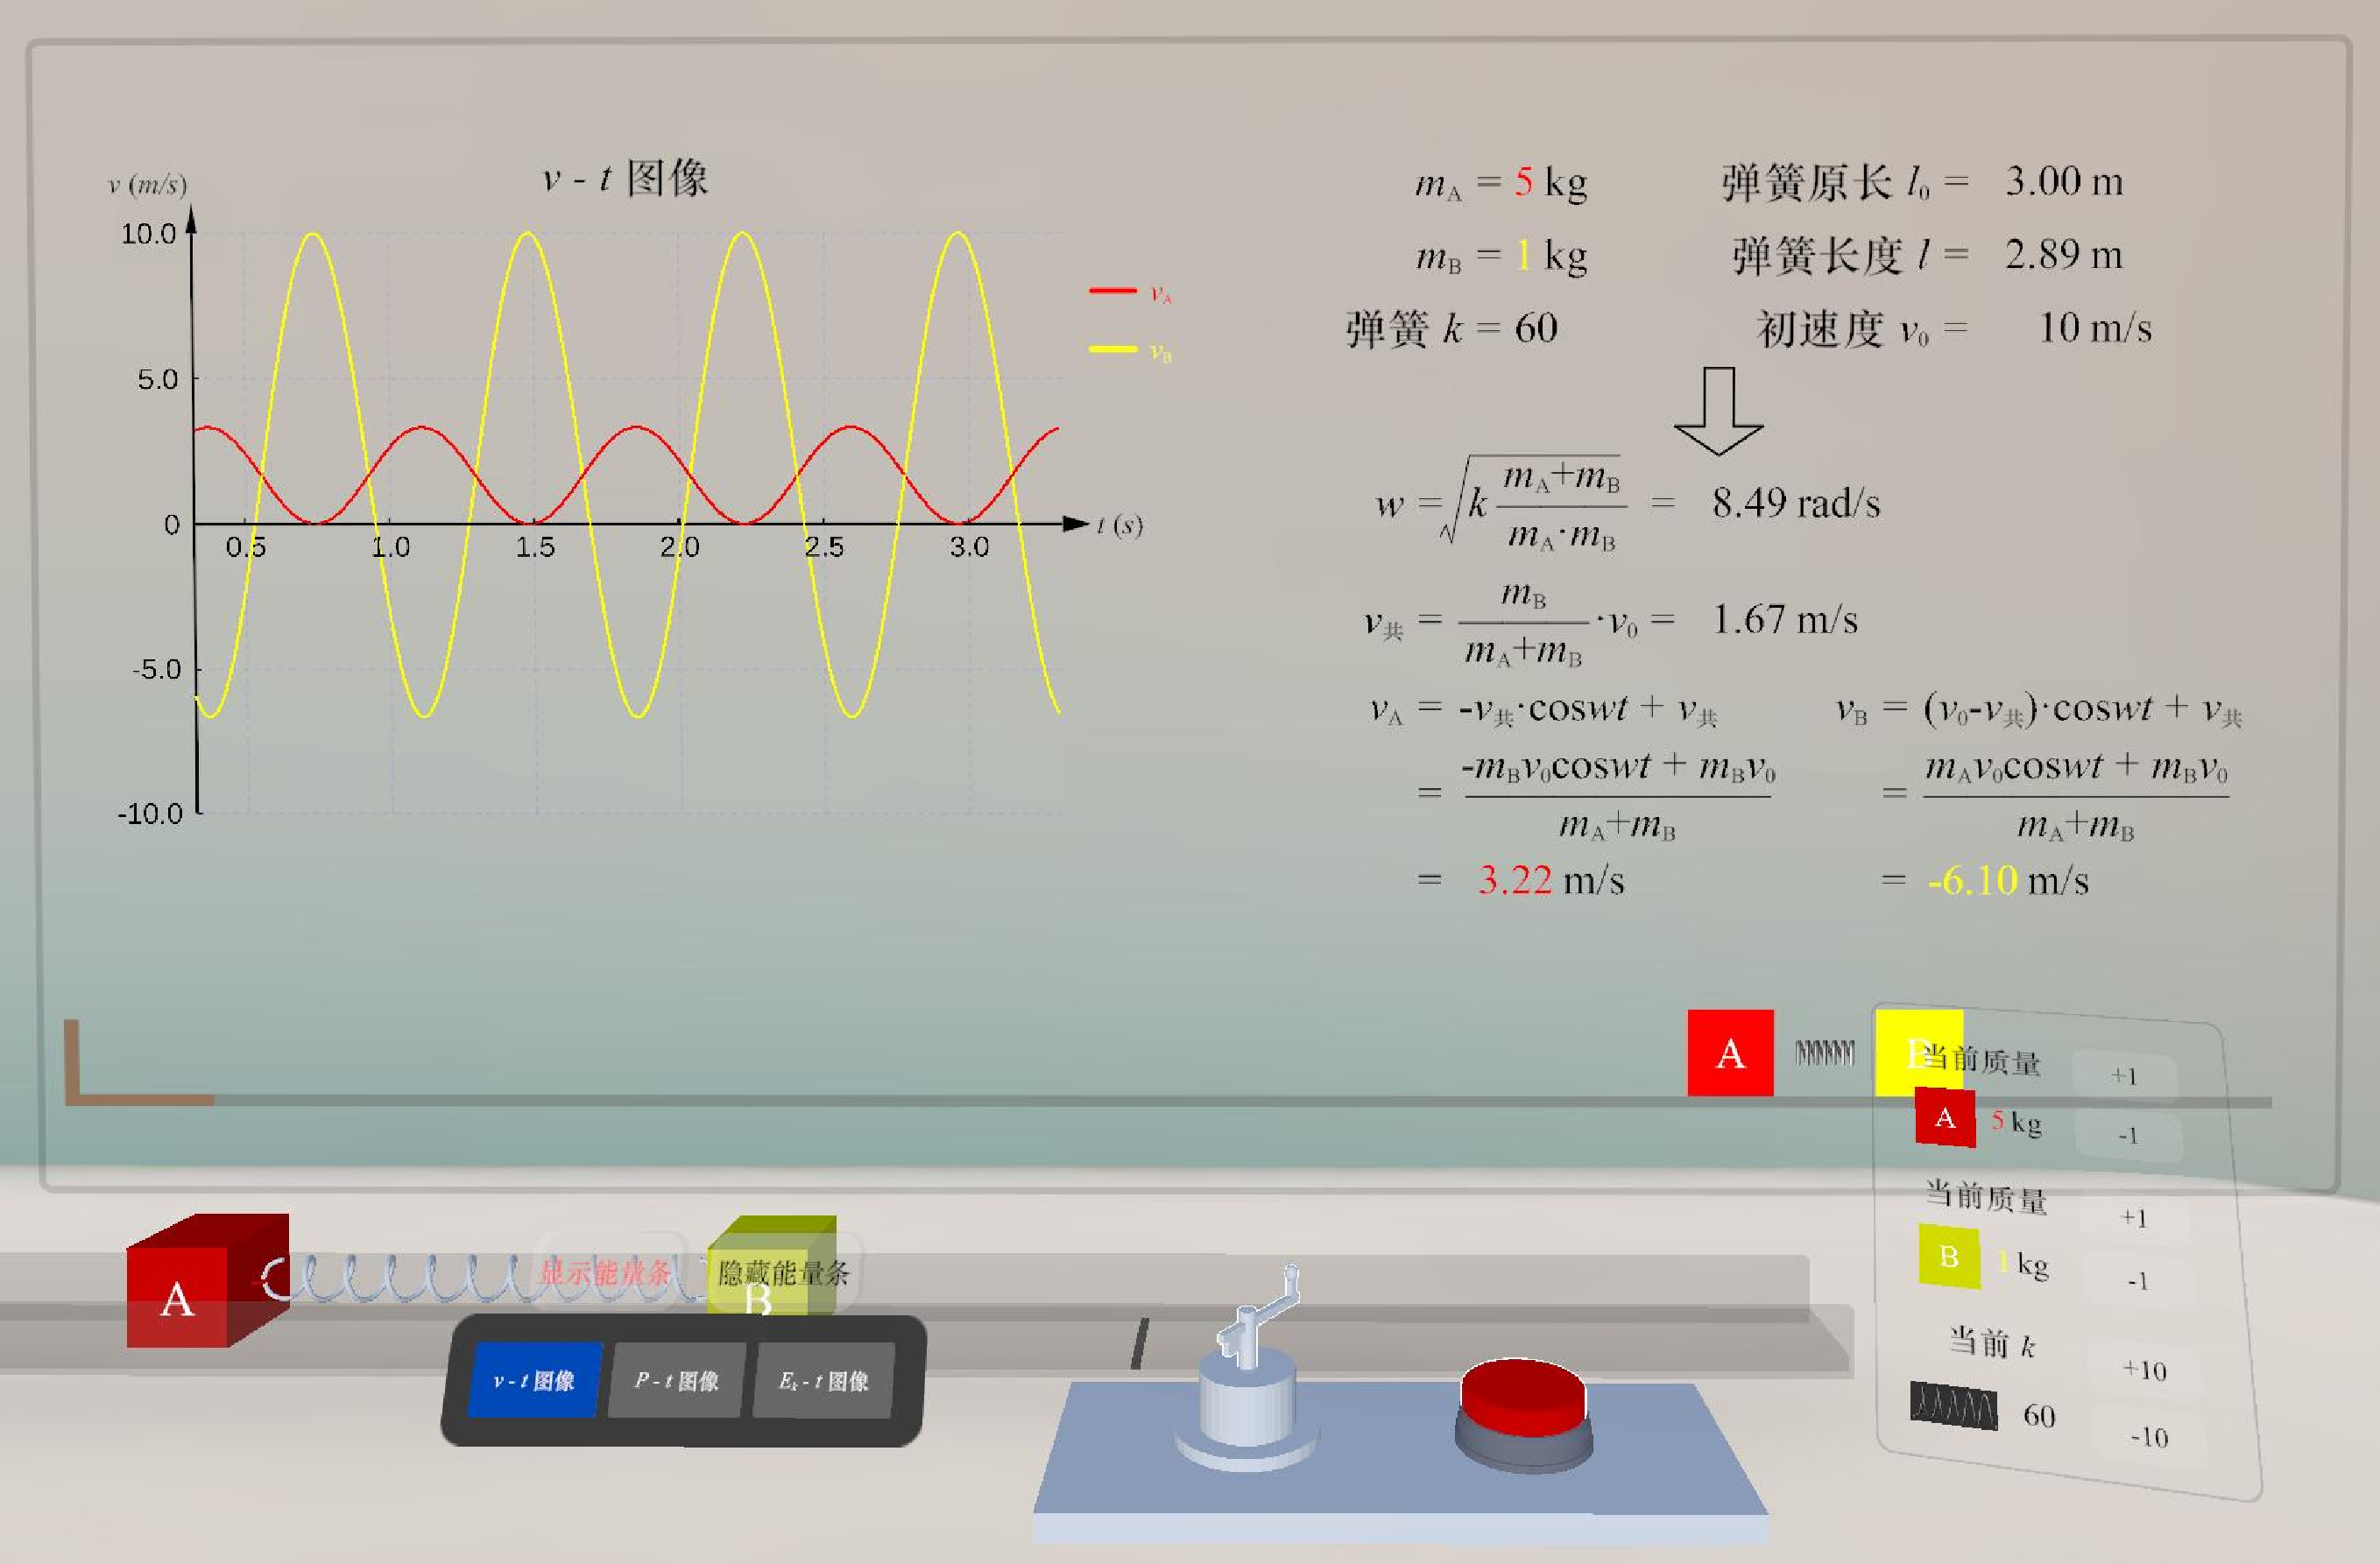
\includegraphics[width=\linewidth]{image/experiment-scenario.pdf}
  \caption{Experimental scenario}
  \label{fig:experimental-operation}
 \end{subfigure}
 \caption{The experimental environment. (\subref{fig:experimental-introduction}) The evaluation environment, (\subref{fig:experimental-operation}) The experimental scenario.}
 \label{fig:experimental-show}
\end{figure}

\begin{enumerate}[label={$\bullet$}]
 \item \texttt{Hardware} Meta Quest 3 VR headset, 3D-printed interactive entity with integrated sensors.
 \item \texttt{Software} Virtual experiment scene developed with Unity 2021.3, including a parameter adjustment panel and a data visualization interface.
 \item \texttt{Data Collection Tools} Knowledge test questionnaire, subjective questionnaires, SynAmps2 amplifier (sampling rate 1000Hz), Gelfree Net Cap saline-based EEG cap.
\end{enumerate}

\subsection{Experimental Content and Procedure}
\subsubsection{Experimental Content}
The core task was the "Verification of the Law of Conservation of Momentum." First, students adjusted the mass of blocks A and B (100-500g) and the spring constant (10-100N/m) using buttons. Second, they grasped the slider of a pulling device, pulled it back to a specified mark (0-10cm), and then released it to observe the two blocks spring apart. Third, they replayed the experiment by turning a knob and verified the conservation law using v-t (velocity-time) and P-t (momentum-time) graphs on a virtual panel. Finally, they reset the experiment by pressing a button, recorded the experimental data, and answered a knowledge test questionnaire.

\subsubsection{Group Design}
Using simple random sampling, participants were divided into an experimental group and a control group, with 32 participants in each. The experimental group (n=32) used gesture interaction while simultaneously manipulating both the virtual object and a 3D-printed interactive entity, receiving both visual and haptic feedback. The control group (n=32) used gesture interaction to manipulate the virtual object, receiving only visual feedback.

\subsubsection{Experimental Procedure}
First, demographic information and prior experience with VR devices and haptic feedback equipment were collected from the students, who were then assigned to either the experimental or control group. A pre-test on relevant physics concepts was then administered. Before the formal experiment, each student practiced using the equipment, watched a demonstration video of the entire interactive task, and carefully read and signed an informed consent form. Meanwhile, researchers calibrated the EEG system, fitted the participant with an EEG cap, applied conductive gel, and had them wear the VR headset. Throughout the experiment, researchers supervised the process to ensure participants followed the procedure and to record experimental data. After the experiment, each student was given questionnaires to fill out, including the knowledge post-test and cognitive load scales.

\subsection{Measurement Metrics}
\subsubsection{Physics Knowledge Test}
The physics knowledge test was provided by Professor XXX and his team from the Department of Physics at XXX University. It was divided into a pre-test and a post-test, each consisting of 10 items worth 1 point each, for a total of 10 points. Both tests were composed of classic high school physics questions covering the basic concepts, formula derivations, and applications of the law of conservation of momentum. The test formats were multiple-choice and fill-in-the-blank questions. The knowledge points tested were identical, with only the phrasing being different between the two tests.

\subsubsection{Subjective Questionnaires}
All questionnaires used were 5-point Likert scales. Cognitive load was measured using the Klepsch scale\cite{klepsch2017development}, which includes three dimensions: Intrinsic Cognitive Load (ICL), Extraneous Cognitive Load (ECL), and Germane Cognitive Load (GCL). Learning motivation was measured using Keller's ARCS model scale\cite{keiier1987systematic}, covering four dimensions: Attention, Relevance, Confidence, and Satisfaction. Immersion was measured using the Schubert scale\cite{schubert2001experience}, which includes three dimensions: Spatial Presence (SP), Involvement, and Realism. All scales were translated and localized to ensure their suitability for the cultural and educational context of this experiment.

\subsubsection{Objective Physiological Metrics}
Objective physiological metrics were the electrical signals from key brain regions such as Fz, Cz, Pz, and Oz, collected by a 64-channel EEG system. Relevant studies have shown a significant positive correlation between a learner's cognitive load level and energy changes in specific frequency bands of the EEG signal, such as the $\alpha$ wave (8–13 Hz) and $\theta$ wave (4–8 Hz), as shown in Table~\ref{tab:1}. This study used Power Spectral Density (PSD) estimation based on the classic Welch's method in the EEG field to reveal changes in neural activity states.

\begin{table}
  \centering
  \setlength{\tabcolsep}{2pt} % Increase column spacing (default is 6pt)
  \caption{Experimental Studies on Cognitive Load}
  \begin{tabularx}{\textwidth}{C{0.5} C{0.15} C{0.15} C{0.15}}
    \toprule
    \textbf{Paradigm} & \textbf{Channels} & \textbf{Frequency Bands} & \textbf{Correlation} \\
    \midrule
    N-back  experiment\cite{pergher2019mental} & Fz, Cz, Pz & $\alpha$, $\theta$ & Positive\\
    \addlinespace
    Letter memory experiment\cite{bashivan2015single} & 64-channel & $\theta$, $\alpha$, $\beta$ & Positive \\
    \addlinespace
    Image memory experiment\cite{zhang2016functional} & \makecell{16-channel \\ (mainly Fz)} & $\theta$ & Positive \\
    \addlinespace
    Mathematical calculation experiment\cite{so2017evaluation} & Fp1 & $\theta$ & Positive \\
    \bottomrule
  \end{tabularx}
  \label{tab:1}
\end{table}

\section{Results and Analysis}
\subsection{Physics Knowledge Test}
A Shapiro-Wilks test on the data from the experimental and control groups showed that neither followed a normal distribution. Therefore, the Mann-Whitney U test was used to analyze the differences between the groups. In the following data, a significance level of $p \le 0.05$ (*) indicates a significant difference, $p \le 0.01$ (**) indicates a highly significant difference, and $p \le 0.001$ (***) indicates an extremely significant difference. The effect size is interpreted according to Cohen's criteria: |r|=0.1 is a small effect, 0.3 is a medium effect, and 0.5 is a large effect.

\subsubsection{Pre-test Results}
The experimental and control groups showed no significant difference in the pre-test (p=0.834). Therefore, it can be concluded that the prior physics knowledge level of the two groups was basically the same.

\subsubsection{Post-test Results}
Table \ref{tab:learning-effect} shows the performance of the two groups in the post-test. The overall mean improvement score of the experimental group (1.156 points) was slightly higher than that of the control group (0.656 points), but it did not reach a significant level, with a medium effect size. This indicates that haptic feedback has a positive trend in improving overall physics knowledge, but has not yet formed a statistically significant difference. The interquartile range of the improvement score in the experimental group (2 points) was larger than that of the control group (1 point), suggesting greater variability in the improvement among students in the experimental group, which may be related to factors such as individual adaptability to the teaching intervention and prior physics knowledge.

\begin{table*}[t]
\centering
\setlength{\tabcolsep}{10pt} % Increase column spacing (default is 6pt)
\caption{Mann-Whitney U Test Results for Pre-test to Post-test Improvement Between the Two Groups}
\label{tab:learning-effect}
\begin{tabularx}{\textwidth}{cccccccc}
\toprule
\textbf{Group} & \textbf{Mean(SD)} & \textbf{Q2(Q1,Q3)} & \textbf{U} & \textbf{Z} & \textbf{p} & \textbf{|r|} \\
\midrule

Exp. & 1.156(1.749) & 1(0,2) & \multirow{2}{*}{389} & \multirow{2}{*}{-1.714} & \multirow{2}{*}{0.087} & \multirow{2}{*}{0.303} \\
% \addlinespace
Con. & 0.656(1.33) & 1(0,1) \\
\bottomrule
\end{tabularx}
\caption*{Note: Q2 is the median, Q1 and Q3 are the lower and upper quartiles, respectively.}
\end{table*}

\subsection{Subjective Questionnaires}
Figure \ref{fig:user-experience-result} compares the differences between the two groups in terms of cognitive load, learning motivation, and immersion. The solid dots above each group represent sample points, and the kernel density estimate curve describes their distribution. The box plot below shows the 25\% (Q1), 50\% (Q2), and 75\% (Q3) quartiles. The experimental group showed a significant improvement in learning motivation ($Z=-3.509, p<0.001, |r|=0.620$) and immersion ($Z=-4.751, p<0.001, |r|=0.840$), with a large effect size. At the same time, the total cognitive load of the experimental group and the control group was basically the same ($Z=-0.521, p=0.602, |r|=0.092$), with no significant difference.

\begin{figure*}[t]
  \centering
  \includegraphics[width=0.75\textwidth]{image/user-experience-result.pdf}
  \caption{Comparison of the results for cognitive load, learning motivation, and immersion between the two groups}
  \label{fig:user-experience-result}
\end{figure*}

\subsubsection{Cognitive Load}
The specific differences in cognitive load between the two groups are shown in Table \ref{tab:cognitive-load}. There was no significant difference in total cognitive load, but the sub-dimensions showed differential characteristics. In terms of intrinsic cognitive load, there was no significant difference between the experimental and control groups, which is consistent with the view in cognitive load theory that "intrinsic load is determined by the complexity of the task itself"—both groups completed the same physics experiment task, so the cognitive resource consumption due to the inherent difficulty of the task was comparable. In terms of extraneous cognitive load, the experimental group's score was significantly lower than that of the control group, with a large effect size. This indicates that the introduction of haptic feedback reduced interference from redundant information in the virtual environment, lowering unnecessary consumption of cognitive resources. Germane cognitive load, however, showed the opposite trend: the experimental group was significantly higher than the control group. This result suggests that the multisensory integration of haptic and visual feedback promoted the construction of cognitive schemas—students, through the linked experience of "feeling the pulling force - spring deformation - momentum change," more efficiently integrated new information with existing physics knowledge (such as Hooke's Law and momentum formulas), forming a more stable knowledge schema. Therefore, haptic feedback optimized the allocation of cognitive resources by "reducing extraneous load and increasing germane load" without increasing the overall cognitive burden, thus providing favorable conditions for deep learning.

\begin{table}[t]
\centering
\setlength{\tabcolsep}{2.8pt} % Increase column spacing (default is 6pt)
\caption{Mann-Whitney U Test Results for Cognitive Load Between the Two Groups}
\label{tab:cognitive-load}
\begin{tabularx}{\textwidth}{
  % C{0.1} C{0.14} C{0.18} C{0.22} C{0.08} C{0.08} C{0.08} C{0.08}
  cccccccc
  }
\toprule
\textbf{Category} & \textbf{Group} & \textbf{Mean(SD)} & \textbf{Q2(Q1,Q3)} & \textbf{U} & \textbf{Z} & \textbf{p} & \textbf{|r|} \\
\midrule
\multirow{2}{*}{ICL} 
& Exp. & 2.594(1.072) & 2.5(1.5,3.5) & \multirow{2}{*}{459.5} & \multirow{2}{*}{-0.720} & \multirow{2}{*}{0.472} & \multirow{2}{*}{0.127} \\
& Con. & 2.719(0.902) & 2.25(2,3.5) \\
\addlinespace
\multirow{2}{*}{ECL} 
& Exp. & 1.479(0.301) & 1.333(1,1.917) & \multirow{2}{*}{254} & \multirow{2}{*}{-3.538} & \multirow{2}{*}{<0.001\(^{***}\)} & \multirow{2}{*}{0.625} \\
& Con. & 2.104(0.641) & 2(1.667,2.333) \\
\addlinespace
\multirow{2}{*}{GCL} 
& Exp. & 4.208(0.622) & 4.333(4,4.667) & \multirow{2}{*}{268} & \multirow{2}{*}{-3.337} & \multirow{2}{*}{<0.001\(^{***}\)} & \multirow{2}{*}{0.590} \\
& Con. & 3.708(0.55) & 4(3.333,4) \\
\addlinespace
\multirow{2}{*}{Total} 
& Exp. & 2.781(0.185) & 2.75(2.531,3) & \multirow{2}{*}{473.5} & \multirow{2}{*}{-0.521} & \multirow{2}{*}{0.602} & \multirow{2}{*}{0.092} \\
& Con. & 2.859(0.252) & 2.75(2.625,3.219) \\
\bottomrule
\end{tabularx}
\end{table}

\subsubsection{Learning Motivation}
As shown in Table \ref{tab:learning-motivation}, the experimental group scored significantly higher than the control group in attention, relevance, confidence, satisfaction, and overall learning motivation, with effect sizes ranging from medium to large. Analyzing from the perspective of the ARCS motivation model: in the attention dimension, the experimental group was significantly better, indicating that the "novelty of operation" brought by haptic feedback (e.g., changes in resistance when pulling) was more effective at keeping students focused on the experimental process. In the relevance dimension, the experimental group scored higher because the realistic tactile sensations made it easier for students to connect the virtual experiment with life experiences and perceive the practical value of the learning content. In the confidence dimension, the experimental group performed better, which is related to haptic feedback reducing operational difficulty—students could confirm the effectiveness of their operations through physical contact, reducing "anxiety about misoperation." In the satisfaction dimension, the experimental group's advantage was most significant, suggesting that the dual "haptic-visual" feedback after successfully completing the experiment brought a stronger sense of accomplishment.

\begin{table*}[t]
\centering
\setlength{\tabcolsep}{3.4pt} % Increase column spacing (default is 6pt)
\caption{Mann-Whitney U Test Results for Dimensions of Learning Motivation Between the Two Groups}
\label{tab:learning-motivation}
\begin{tabularx}{\textwidth}{cccccccc}
\toprule
\textbf{Category} & \textbf{Group} & \textbf{Mean(SD)} & \textbf{Q2(Q1,Q3)} & \textbf{U} & \textbf{Z} & \textbf{p} & \textbf{|r|} \\
\midrule
\multirow{2}{*}{Attention} 
& Exp. & 4.667(0.323) & 5(4.333,5) & \multirow{2}{*}{271} & \multirow{2}{*}{-3.382} & \multirow{2}{*}{0.001\(^{***}\)} & \multirow{2}{*}{0.598} \\
& Con. & 4.01(0.892) & 4(3.75,4.917) \\
\addlinespace
\multirow{2}{*}{Relevance} 
& Exp. & 4.672(0.494) & 5(4.5,5) & \multirow{2}{*}{287.5} & \multirow{2}{*}{-3.313} & \multirow{2}{*}{0.001\(^{***}\)} & \multirow{2}{*}{0.586} \\
& Con. & 4(1.145) & 4(3.625,5) \\
\addlinespace
\multirow{2}{*}{Confidence} 
& Exp. & 4.563(0.544) & 5(4,5) & \multirow{2}{*}{303.5} & \multirow{2}{*}{-3.001} & \multirow{2}{*}{0.003\(^{**}\)} & \multirow{2}{*}{0.531} \\
& Con. & 3.906(1.072) & 4(3.625,5) \\
\addlinespace
\multirow{2}{*}{Satisfaction} 
& Exp. & 4.573(0.167) & 4.667(4.333,5) & \multirow{2}{*}{210} & \multirow{2}{*}{-4.127} & \multirow{2}{*}{<0.001\(^{***}\)} & \multirow{2}{*}{0.730} \\
& Con. & 3.917(0.466) & 4(3.667,4.333) \\
\addlinespace
\multirow{2}{*}{Total} 
& Exp. & 4.619(0.278) & 4.8(4.275,5) & \multirow{2}{*}{252.5} & \multirow{2}{*}{-3.509} & \multirow{2}{*}{<0.001\(^{***}\)} & \multirow{2}{*}{0.620} \\
& Con. & 3.959(0.701) & 4(3.525,4.675) \\
\bottomrule
\end{tabularx}
\end{table*}

\subsubsection{Immersion}
As shown in Table \ref{tab:immersion}, the experimental group scored significantly higher than the control group in spatial presence, involvement, realism, and overall immersion, with generally large effect sizes. From the dual-dimensional perspective of immersion theory: at the physical/sensory immersion level, the significant differences in spatial presence and realism were most prominent. Because the "touched pulling device moved in sync with the seen virtual slider," students in the experimental group were more likely to experience the spatial illusion of "being in a real laboratory." In contrast, the control group, perceiving the virtual object only through vision, found it difficult to establish a stable spatial anchor. At the psychological immersion level, the difference in the involvement dimension indicates that the experimental group was more likely to enter a state of "deep engagement." This is related to haptic feedback reducing cognitive distraction—students did not need to frequently recalibrate their gestures, allowing more attention to be focused on core tasks like "observing the law of momentum change," thereby extending their concentration duration. This high level of immersion further reinforced the positive feedback loop between learning motivation and cognitive engagement.

\begin{table*}[t]
\centering
\setlength{\tabcolsep}{2.4pt} % Increase column spacing (default is 6pt)
\caption{Mann-Whitney U Test Results for Dimensions of Immersion Between the Two Groups}
\label{tab:immersion}
\begin{tabularx}{\textwidth}{cccccccc}
\toprule
\textbf{Category} & \textbf{Group} & \textbf{Mean(SD)} & \textbf{Q2(Q1,Q3)} & \textbf{U} & \textbf{Z} & \textbf{p} & \textbf{|r|} \\
\midrule
\multirow{2}{*}{SP} 
& Exp. & 4.55(0.206) & 4.6(4.2,5) & \multirow{2}{*}{179} & \multirow{2}{*}{-4.524} & \multirow{2}{*}{<0.001\(^{***}\)} & \multirow{2}{*}{0.800} \\
& Con. & 3.637(0.842) & 3.8(3.2,4.2) \\
\addlinespace
\multirow{2}{*}{Involvement} 
& Exp. & 3.484(0.342) & 3.5(3,3.938) & \multirow{2}{*}{307.5} & \multirow{2}{*}{-2.774} & \multirow{2}{*}{0.006\(^{**}\)} & \multirow{2}{*}{0.490} \\
& Con. & 2.961(0.488) & 3(2.313,3.5) \\
\addlinespace
\multirow{2}{*}{Realism} 
& Exp. & 3.74(0.442) & 3.667(3.333,4.333) & \multirow{2}{*}{210} & \multirow{2}{*}{-4.102} & \multirow{2}{*}{<0.001\(^{***}\)} & \multirow{2}{*}{0.725} \\
& Con. & 2.875(0.593) & 3(2.417,3.333) \\
\addlinespace
\multirow{2}{*}{Total} 
& Exp. & 3.992(0.156) & 4(3.688,4.333) & \multirow{2}{*}{159} & \multirow{2}{*}{-4.751} & \multirow{2}{*}{<0.001\(^{***}\)} & \multirow{2}{*}{0.840} \\
& Con. & 3.221(0.469) & 3.292(2.771,3.646) \\
\bottomrule
\end{tabularx}
\end{table*}

\subsection{Neurophysiological Signals}
By selecting the Fz, Cz, Pz, and Oz electrode channels, performing PSD estimation on the electrical signals, and finally calculating the average power, the results are as shown in Table~\ref{tab:3}.

\begin{table}[t]
\centering
\setlength{\tabcolsep}{15pt} % Increase column spacing (default is 6pt)
\caption{Comparison of Average Power in Different Frequency Bands Across Brain Regions}
\label{tab:3}
\begin{tabularx}{\textwidth}{ccccc}
\toprule
\textbf{\makecell{Brain Region \\ (Channel)}} & \textbf{Band} & \textbf{\makecell{Overall \\ (Pre)}} & \textbf{\makecell{Exp. \\ (Post)}} & \textbf{\makecell{Con. \\ (Post)}} \\
\midrule
\multirow{3}{*}{Frontal Lobe (Fz)} & $\theta$ & 1.78 & 1.64 & 2.55 \\
 & $\alpha$ & 0.68 & 0.64 & 0.74 \\
 & $\beta$ & 0.32 & 0.17 & 0.26 \\
\addlinespace
\multirow{3}{*}{Central Sulcus (Cz)} & $\theta$ & 1.62 & 0.88 & 1.15 \\
 & $\alpha$ & 0.69 & 0.49 & 0.58 \\
 & $\beta$ & 0.26 & 0.13 & 0.19 \\
\addlinespace
\multirow{3}{*}{Parietal Lobe (Pz)} & $\theta$ & 2.02 & 1.44 & 1.53 \\
 & $\alpha$ & 1.25 & 0.97 & 0.96 \\
 & $\beta$ & 0.48 & 0.37 & 0.33 \\
\addlinespace
\multirow{3}{*}{Occipital Lobe (Oz)} & $\theta$ & 3.49 & 2.70 & 4.23 \\
 & $\alpha$ & 3.76 & 2.79 & 2.84 \\
 & $\beta$ & 2.13 & 1.85 & 1.54 \\
\bottomrule
\end{tabularx}
\caption*{Note: The unit is $\mu V^2$.}
\end{table}

The EEG signal analysis shows that in the Fz, Cz, Pz, and Oz electrode channels, the average power in the $\theta$, $\alpha$, and $\beta$ bands for the experimental group showed a downward trend, and the magnitude of the decrease was generally greater than that of the control group. Conversely, the control group showed an increase in the average power of the $\alpha$ wave in the Fz and Oz channels. For example, in the Fz channel, the post-test $\theta$ wave power for the experimental group was 1.64, significantly lower than the control group's 2.55 and lower than the pre-test value of 1.78. Similarly, in the Oz channel, the experimental group's $\theta$ wave power decreased to 2.70, while the control group's increased to 4.23.
In cognitive neuroscience research, the frontal lobe is responsible for higher cognitive functions such as problem-solving, decision-making, working memory, and attention regulation, while the occipital lobe is responsible for advanced visual functions like analyzing color, shape, motion direction, and integrating visual memories\cite{kolb2009fundamentals}. The results indicate that the brains of learners in the control group may face greater pressure in allocating neural resources when performing the learning task. The haptic feedback interaction experienced by the students in the experimental group effectively reduced their cognitive load, whereas the gesture-only interaction of the control group students may have caused additional cognitive load. Haptic feedback interaction helps to alleviate the load on the frontal lobe region and optimize cognitive resource allocation, thereby enabling students to learn more easily during the experiment and improving the efficiency and quality of information processing.

\section{Discussion and Implications}
\subsection{Discussion of Results}
\subsubsection{The Impact of Haptic Feedback on Knowledge Acquisition} 
Hypothesis H1 proposed that "appropriate haptic feedback can improve learners' knowledge acquisition." The experimental results showed that the improvement score of the experimental group in the post-test was slightly higher than that of the control group (mean 1.156 vs. 0.656), presenting a medium effect size (|r|=0.303), but it did not reach a statistically significant level (p=0.087). Therefore, this hypothesis is considered not supported for now.

This "positive trend but not significant" result can be explained from three aspects:

\begin{enumerate}[label={\arabic*)}]
 \item \texttt{Limitations of Short-Term Intervention} The experimental task focused on a single knowledge point, the "verification of the law of conservation of momentum," and the duration of the single intervention was limited. The deep internalization of knowledge through haptic feedback may require a longer period—the neural pathways formed by multisensory integration need repeated reinforcement to be transformed into stable knowledge representations. Future research could extend the intervention period to observe long-term learning effects.
 \item \texttt{Sensitivity of Knowledge Measurement} The current test primarily used multiple-choice and fill-in-the-blank questions, focusing on knowledge recognition and recall. The advantage of haptic feedback may lie in the intuitive construction of concepts (such as "the connection between the action of force and the change in momentum"), and this type of deep understanding needs to be further measured through open-ended questions or operational tasks.
 \item \texttt{Moderating Role of Individual Differences} The interquartile range of the improvement score in the experimental group (2 points) was larger than that of the control group (1 point), suggesting that the effect of haptic feedback may be influenced by individual traits such as learners' spatial cognitive abilities and hands-on operational experience. Subsequent studies could use regression analysis to explore moderating variables, providing a basis for personalized feedback design.
\end{enumerate}

Despite not reaching a significant level, the medium effect size still indicates that haptic feedback has a positive impact on knowledge learning, which needs to be further verified with a larger sample size.

\subsubsection{The Optimization Mechanism of Haptic Feedback on Interactive Experience}
Hypothesis H2 proposed that "appropriate haptic feedback can enhance learners' interactive experience," and the experimental results provide strong support for this. The experimental group showed significant improvements in learning motivation and immersion, and a more optimal cognitive load structure. Therefore, we consider this hypothesis to be supported, and its internal mechanism is analyzed as follows:

\begin{enumerate}[label={\arabic*)}]
 \item \texttt{Structural Optimization of Cognitive Load} The extraneous cognitive load of the experimental group was significantly reduced, while the germane cognitive load was significantly increased, with the total load remaining unchanged. This result is consistent with cognitive load theory—haptic feedback, by optimizing interaction, reduces the extraneous load required to process irrelevant task elements, while promoting the integration of multiple representations to increase germane load, ultimately achieving efficient allocation of cognitive resources.
 \item \texttt{Analysis via the ARCS Model of Motivation} In terms of Attention, the "novelty" of haptic feedback continuously activates the attention network through peripheral nerve stimulation, avoiding fatigue caused by single visual input. In terms of Relevance, realistic tactile sensations connect abstract physical quantities (like the spring constant) with life experiences (like the feel of pulling a rubber band), enhancing the perceived "usefulness" of the knowledge. In terms of Confidence, haptic feedback reduces the "uncertainty" of virtual operations (such as confirming that the slider has been pulled to the specified mark), reducing operational anxiety. In terms of Satisfaction, the dual "haptic-visual" feedback strengthens the "closed-loop" sense of the operation, making the sense of accomplishment from a successful experiment more intense.
 \item \texttt{Multi-dimensional Enhancement of Immersion} The large effect size of the experimental group in spatial presence and environmental realism confirms the view that "haptic feedback is a core cue for establishing a sense of reality in a virtual environment." The synchronized movement of the 3D-printed entity and the virtual object (the resistance feedback when pulling the slider) provides a stable "sensory anchor" for the learner, reducing the "floating sensation" unique to vision, thereby enhancing the spatial illusion of "being in a real laboratory."
\end{enumerate}

\subsection{Educational Implications}
\subsubsection{Implications for Virtual Experiment Instructional Design}
Haptic feedback should follow a principle of "appropriateness"; it is not the case that the higher the feedback intensity, the better the effect. "Just right" haptic cues should be designed based on the characteristics of the knowledge point. For example, in the momentum conservation experiment, the resistance feedback of the pulling device should be strictly matched with the spring constant of the virtual spring to avoid excessive feedback interfering with the perception of physical laws. Furthermore, in response to the large variation in improvement within the experimental group, an adaptive feedback system could be designed. For learners with operational difficulties, increased haptic guidance could be provided to reduce extraneous load; for more capable learners, haptic challenges with variable parameters could be offered to increase germane load.

\subsubsection{Implications for Secondary School Physics Teaching Practice}
First, the abstract nature of physical quantities like momentum and force is a teaching difficulty. With the help of haptic feedback, "change in momentum" can be transformed into a "sensation of impulse on the hand," and "spring constant" can be transformed into "differences in resistance when pulling," helping students build "embodied cognition." Second, traditional physics experiments are limited by equipment cost or safety, whereas VR + haptic feedback can simulate hazardous scenarios, allowing students to gain "immersive operational" experience in a safe environment. Finally, the high effect size of the experimental group in the satisfaction dimension suggests that the "pleasure" brought by haptic feedback can be converted into motivation for continuous learning. Teachers can use such virtual experiments as pre-class previews or post-class extension tools to compensate for the interactive limitations of traditional classrooms.

\subsubsection{Implications for Educational Technology Development}
First, current 3D-printed interactive entities still have issues of high customization costs and insufficient portability. In the future, modular haptic devices could be developed to lower the application threshold for schools. Second, this study did not deeply analyze neurophysiological signals; future research could explore the impact of haptic feedback on brain activation patterns to provide a basis for the design of neuroeducation. Finally, the design of haptic feedback in physics experiments requires the integration of knowledge from multiple disciplines such as physics and psychology. In the future, a collaborative R\&D mechanism of "educational technology - subject teaching - engineering design" could be established.

\section{Conclusion}
This study, using the high school physics experiment "Verification of the Law of Conservation of Momentum" as a vehicle, systematically investigated the impact of haptic feedback on physics learning outcomes in immersive gesture-based learning environment. By integrating and analyzing multimodal data from physics knowledge tests, subjective questionnaires, and objective physiological metrics, it systematically explored the differential effects of haptic feedback on interactive experience and knowledge acquisition. The research results indicate that introducing haptic feedback into a virtual experiment scenario, although not producing a statistically significant improvement in learners' knowledge acquisition (p=0.087), showed a positive trend with a medium effect size. At the same time, it significantly enhanced learners' learning motivation (p<0.001) and immersion (p<0.001), and achieved a structural optimization of cognitive resources by reducing extraneous cognitive load and increasing germane cognitive load, without increasing the overall cognitive burden (p=0.602). These findings provide empirical evidence for understanding the value of multisensory interaction in immersive learning and open up new perspectives for the innovative integration of educational technology and subject teaching.

Future research could be extended to more subject areas (such as mechanics and electromagnetism) and involve longer intervention periods to verify the long-term effects and cross-disciplinary applicability of haptic feedback. Additionally, as the knowledge test in this study primarily consisted of recognition and recall items, subsequent studies could include open-ended questions and problem-solving tasks to more accurately assess deep understanding.

\begin{credits}
\subsubsection{\ackname} 
This research was supported by the National Natural Science Foundation of China (NSFC) under Grant No. XXX.

\subsubsection{\discintname}
The authors declare no conflict of interest.
\end{credits}

\bibliography{VRTI-bib}

\end{document}